%!TEX root = ../thesis.tex

\centering
  \begin{subfigure}[b]{0.98\textwidth}
    \centering
      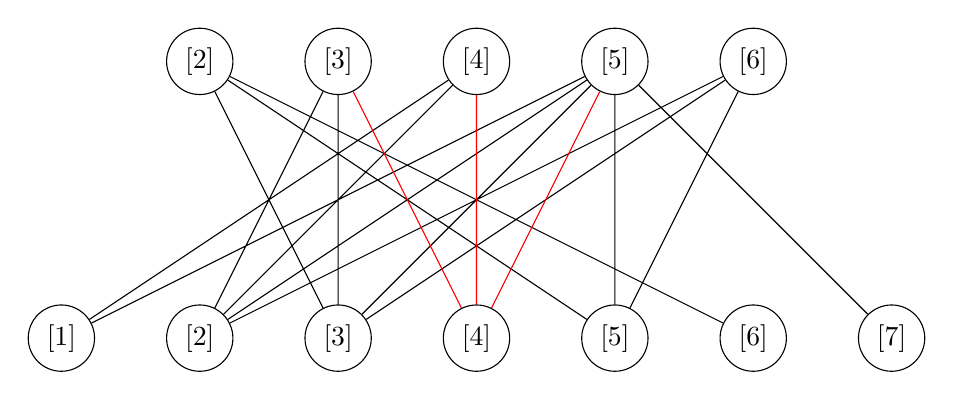
\begin{tikzpicture}
        {\tikzstyle{every node}=[circle, draw]
          \foreach \i in {2, ..., 6}
          {
            \node (s\i) at (\i*50pt, 100pt) {\species[\i]};
          }

          \foreach \j in {1, ..., 7}
          {
            \node (c\j) at (\j*50pt, 0) {\character[\j]};
          }
        }

        \draw
          (c1) -- (s4)
          (c1) -- (s5)
          (c2) -- (s3)
          (c2) -- (s4)
          (c2) -- (s5)
          (c2) -- (s6)
          (c3) -- (s2)
          (c3) -- (s3)
          (c3) -- (s5)
          (c3) -- (s6)
          (c5) -- (s2)
          (c5) -- (s5)
          (c5) -- (s6)
          (c6) -- (s2)
          (c7) -- (s5);

        \draw[red]
          (c4) -- (s3)
          (c4) -- (s4)
          (c4) -- (s5);
      \end{tikzpicture}

    \caption{Red-black graph \grb{}}
    \label{figure:5:a}
  \end{subfigure}

  \bigskip

  \begin{subfigure}[b]{0.98\textwidth}
    \centering
      \begin{tabular}{l | l}
        \character[i] & $S(\character[i])$ \\ \hline
        \character[1] & $\{ \species[4], \species[5] \}$ \\
        \character[2] & $\{ \species[3], \species[4], \species[5], \species[6] \}$ \\
        \character[3] & $\{ \species[2], \species[3], \species[5], \species[6] \}$ \\
        \character[5] & $\{ \species[2], \species[5], \species[6] \}$ \\
        \character[6] & $\{ \species[2] \}$ \\
        \character[7] & $\{ \species[5] \}$
      \end{tabular}

    \caption{Adjacency lists of the inactive characters in \grb{}}
    \label{figure:5:b}
  \end{subfigure}

  \bigskip

  \begin{subfigure}[b]{0.98\textwidth}
    \centering
      {\renewcommand{\arraystretch}{1.5}
      \begin{tabular}{| l | l | l | l |}
        \hline

        \boldmath $S(\character[i])$, $\character[i] \in \grb{}$ &
        \boldmath $S(\character[j])$, $\character[j] \in \cm{}$ &
        \boldmath $Operation$ &
        \boldmath \cm{} \\

        \hline

        $S(\character[1]) = \{ \species[4], \species[5] \}$ &
        &
        Add \character[1] &
        $\{ \character[1] \}$ \\

        \hline

        $S(\character[2]) = \{ \species[3], \species[4], \species[5], \species[6] \}$ &
        $S(\character[1]) = \{ \species[4], \species[5] \}$ &
        Replace \character[1] &
        $\{ \character[2] \}$ \\

        \hline

        $S(\character[3]) = \{ \species[2], \species[3], \species[5], \species[6] \}$ &
        $S(\character[2]) = \{ \species[3], \species[4], \species[5], \species[6] \}$ &
        Add \character[3] &
        $\{ \character[2], \character[3] \}$ \\

        \hline

        $S(\character[5]) = \{ \species[2], \species[5], \species[6] \}$ &
        $S(\character[2]) = \{ \species[3], \species[4], \species[5], \species[6] \}$ &
        &
        \\

        &
        $S(\character[3]) = \{ \species[2], \species[3], \species[5], \species[6] \}$ &
        Ignore \character[5] &
        $\{ \character[2], \character[3] \}$ \\

        \hline

        $S(\character[6]) = \{ \species[2] \}$ &
        $S(\character[2]) = \{ \species[3], \species[4], \species[5], \species[6] \}$ &
        &
        \\

        &
        $S(\character[3]) = \{ \species[2], \species[3], \species[5], \species[6] \}$ &
        Ignore \character[6] &
        $\{ \character[2], \character[3] \}$ \\

        \hline

        $S(\character[7]) = \{ \species[5] \}$ &
        $S(\character[2]) = \{ \species[3], \species[4], \species[5], \species[6] \}$ &
        &
        \\

        &
        $S(\character[3]) = \{ \species[2], \species[3], \species[5], \species[6] \}$ &
        Ignore \character[7] &
        $\{ \character[2], \character[3] \}$ \\

        \hline
      \end{tabular}}

    \caption{Computation of \cm{} for \grb{}}
    \label{figure:5:c}
  \end{subfigure}
